% =====================================================================================
% Ensembled Transformer-Graph Streams - IEEE conference paper (IEEEtran, 2 columns, ~8 pages)
% Build: pdflatex main -> bibtex main -> pdflatex main -> pdflatex main   (or upload paper/ to Overleaf)
%
% STATUS: step 1 = skeleton (done); step 2 = Data, Methods, Table I, settings table, Fig. 1 (done);
% step 3 = Experimental Setup, Results (main table + McNemar, per-class, survival table, omics importance) (done);
% step 4 = Introduction (contributions) and Related Work (done);
% step 5 = Discussion, Limitations, Conclusion, Data and Code Availability (done);
% step 6 = Abstract and title (done).
% 2026-11-10: one sample per patient (5 duplicate metastatic samples removed, owner decision 1-B); BRCA and COADREAD
% re-run for our model and both released codes; all BRCA/COADREAD numbers updated and checked against the new files
% (old files in results/archive_with_duplicate_samples/).
% Grey italic text (\plan{...}) is the outline of what each part will say;
% it is replaced section by section in steps 2-6. [CITE?] = reference still to be confirmed.
% Red [CHECK: ...] = a statement the owner must confirm or decide before submission.
% Every number in this paper must come from results/ (final_ensembled_streams, baselines_author_code,
% comparison_author_code) and is checked against those files in step 7.
% =====================================================================================
\documentclass[conference]{IEEEtran}
\IEEEoverridecommandlockouts

\usepackage{cite}
\usepackage{amsmath,amssymb}
\usepackage{graphicx}
\usepackage{booktabs}
\usepackage{multirow}
\usepackage{xcolor}
\usepackage{tikz}
\usetikzlibrary{positioning,arrows.meta,fit,backgrounds}
\usepackage[hidelinks]{hyperref}

\newcommand{\plan}[1]{{\color{gray}\itshape [Plan: #1]}}
\newcommand{\citecheck}{{\color{red}[CITE?]}}
\newcommand{\tocheck}[1]{{\color{red}[CHECK: #1]}}

\begin{document}

\title{Ensembled Transformer-Graph Streams for Joint Cancer Subtyping, Survival Prediction and Biological
Interpretation from Multi-Omics Data}
% title chosen by the owner 2026-11-09

\author{
\IEEEauthorblockN{Author 1}
\IEEEauthorblockA{Department \\ Institution \\ City, Country \\ email}
\and
\IEEEauthorblockN{Author 2}
\IEEEauthorblockA{Department \\ Institution \\ City, Country \\ email}
}

\maketitle

% -------------------------------------------------------------------------------------
\begin{abstract}
% Sources: same numbers as Table~\ref{tab:main} (pooled accuracy / macro-F1, McNemar) and Table~\ref{tab:surv}
% (fold-mean C-index, log-rank p); see the source comments of the Results section.
Supervised multi-omics models for cancer subtyping either learn interactions among one patient's features or
similarities between patients, and survival is rarely learned jointly with the subtype. We combine two
published subtype classifiers, a driver-aware transformer and a patient-similarity graph network, as unchanged streams
of one model. Bilateral cross-attention fuses the streams and feeds a subtype head (class-balanced focal loss) and a
Cox survival head. Five bagged members per training fold use disjoint stream, fusion and selection sets and random
feature subspaces, so test patients are never used for model selection. On five TCGA cohorts (BRCA, LGG, KIPAN,
COADREAD, STAD) with mRNA, miRNA and methylation, we re-ran both original codes on identical 5-fold
splits. The ensembled model had the highest pooled accuracy on three cohorts, tied with its graph stream on STAD and
trailed it by one sample on COADREAD (0.7578--0.9801; macro-F1 0.3882--0.9815).
It was significantly better than the released transformer code on all cohorts (McNemar $p\le0.037$) and than the
released graph code on BRCA, LGG and COADREAD, but its difference from its bagged graph stream was small
($-0.0031$ to 0.0089) and not significant. Its risk score reached a mean C-index of 0.662, 0.765 and 0.659 on BRCA, LGG
and KIPAN and separated high- and low-risk patients significantly there (log-rank $p\le0.025$), but not on COADREAD and
STAD (0.564 and 0.532). Single-feature masking ranked known markers such as IDH1 and ATRX (LGG) and FOXC1 and ESR1
(BRCA) highly, although effects were small. Classes with 2 or 7 samples were never predicted
correctly.
\end{abstract}

\begin{IEEEkeywords}
multi-omics integration, cancer subtype classification, survival analysis, transformer, graph neural network, ensemble learning
\end{IEEEkeywords}

% -------------------------------------------------------------------------------------
% Sources: abstracts and method/evaluation sections of the PDFs in papers/ (read 2026-11-08).
% Naming rule: MOTCS and MO-GCAN are named once each (below); everywhere else "transformer method" / "graph method".
\section{Introduction}
Molecular subtypes of a cancer differ in prognosis and in their response to treatment, and large projects such as The
Cancer Genome Atlas (TCGA) have shown that they are reflected across several molecular layers at once
\cite{weinstein2013tcga,hoadley2018pancan}. Supervised models that classify subtypes from several omics of the same
patient are therefore an active area of research.

Two recent families of such models look at the data from different sides. Feature-level models learn interactions
among the features of one patient. MOTCS \cite{meng2026motcs}, for example, treats every feature as a token of a
transformer encoder, encodes cancer driver genes separately from features selected by an L1-penalised SVC, and
combines the omics with a View Correlation Discovery Network. Patient-level models learn from similarities between
patients. MOGONET \cite{wang2021mogonet}, DeepMoIC \cite{wu2024deepmoic} and MO-GCAN \cite{dou2025mogcan} build
patient graphs and classify them with graph neural networks; the last of these extracts latent features with one graph
convolutional network per omics and classifies them with a graph attention network on a fused similarity network
\cite{wang2014snf}.

Three gaps motivate this work. First, the two views are complementary, but published methods use one or the other.
Second, survival is at most analysed after classification, for example as Kaplan--Meier curves of predicted subtypes
\cite{wu2024deepmoic}, rather than learned together with the subtype. Third, methods are usually compared through
published numbers obtained with different omics, labels and evaluation protocols (5-fold cross-validation in
\cite{meng2026motcs}, one 75/25 split in \cite{dou2025mogcan}, one 60/40 split in \cite{wu2024deepmoic}), and the
released code of one of them chooses the training epoch on the test patients.

We therefore combine the two published methods as two streams of one model. Each stream is used as released; a
bilateral cross-attention layer lets each stream's summary attend to the other stream's tokens, and the fused
representation feeds a subtype head and a Cox survival head. Five bagged members per training fold are trained on
disjoint random splits of the training patients, so that the fusion only sees stream outputs of patients the streams
did not train on, and model selection never uses test patients. Our contributions are:
\begin{itemize}
\item a two-stream model that keeps two published subtype classifiers, a driver-aware transformer and a
patient-graph network, unchanged and joins them by bilateral cross-attention with joint subtype and survival training;
\item a bagging scheme with disjoint stream, fusion and selection sets and random feature subspaces;
\item a re-run of both original codes on the same samples, folds and per-fold features as our model, with the epoch of
the transformer code chosen on a validation slice, together with each of our streams alone;
\item an evaluation on five TCGA cohorts (BRCA, LGG, KIPAN, COADREAD, STAD) with paired significance tests, survival
analysis, omics and feature importance and a biological interpretation of the top features, which also reports where
the fusion does not help.
\end{itemize}
The ensembled model has the highest pooled accuracy on three of the five cohorts, ties with its own graph stream on
STAD and is one sample behind it on COADREAD; its difference from its own graph stream alone is small and not
significant on any cohort.

% -------------------------------------------------------------------------------------
\section{Related Work}
\emph{Graph-based integration.} MOGONET \cite{wang2021mogonet} trains one graph convolutional network
\cite{kipf2017gcn} per omics on a patient similarity graph and combines their predictions with a View Correlation
Discovery Network. DeepMoIC \cite{wu2024deepmoic} compresses each omics with autoencoders, builds a patient network by
similarity network fusion \cite{wang2014snf} and classifies it with a deep GCN that uses initial residual connections and
identity mapping. The graph method \cite{dou2025mogcan} keeps only high-confidence edges of the patient graphs, takes the
latent output of a per-omics GCN as features and classifies them with a graph attention network
\cite{velickovic2018gat} on the fused graph.

\emph{Transformer-based integration.} The transformer method \cite{meng2026motcs} applies transformer encoders
\cite{vaswani2017attention} to driver and selected non-driver features of each omics. Subtype-Former
\cite{yang2022subtypeformer} is unsupervised: an MLP--transformer network learns a low-dimensional representation that
is clustered with K-means or consensus clustering, and the subtypes are judged by survival differences.

\emph{Two-stream designs.} Closest to our work, FastMI-HGNet \cite{fu2026fastmi} combines a transformer-based data stream
with a graph attention stream over a heterogeneous sample--feature graph whose edges come from fast mutual information
estimates, and it averages several such models with an uncertainty-aware ensemble. It designs new streams; we instead
keep two complete published methods as streams, add a jointly trained survival head and compare against the original
codes on identical folds.

\emph{Survival and ensembles.} Deep Cox models such as DeepSurv \cite{katzman2018deepsurv} learn a risk score by
minimising the Cox partial likelihood \cite{cox1972}; we use this loss as a second task of the fusion. Bagging
\cite{breiman1996bagging} and the random subspace method \cite{ho1998subspace} reduce the variance of unstable learners,
which matters for cohorts of a few hundred patients.

% -------------------------------------------------------------------------------------
\section{Materials and Methods}

% Sources of every number in this section:
%   data/processed_exact/tcga_<cohort>/preprocessing_metadata.json (samples, labels, classes, deaths, features)
%   logs/preprocess_exact_*.log (CpG counts, imputed values)
%   results/final_ensembled_streams/logs/train_<cohort>.log ("features" line of each fold: driver / L1-SVC counts)
%   data/labels/brca_combined_subtype.tsv (column 'source': 540 PanCancer, 24 Xena PAM50 among the labeled samples)
%   src/preprocess_exact.py, src/train_exact.py, src/models/*.py, external/CHANGES.md (method settings)
\subsection{Data}
\label{sec:data}
We used five TCGA cohorts \cite{weinstein2013tcga} from the UCSC Xena TCGA hub \cite{goldman2020xena}: breast invasive
carcinoma (BRCA), lower-grade glioma (LGG), pan-kidney (KIPAN: KIRC, KIRP and KICH), colorectal adenocarcinoma (COADREAD:
COAD and READ) and stomach adenocarcinoma (STAD). For every TCGA project we downloaded RNA-seq gene expression (HiSeqV2),
miRNA expression (miRNA\_HiSeq\_gene), Illumina 450K DNA methylation and overall survival (OS, OS.time), and recorded size
and SHA-256 checksum of each file. Primary (01) and metastatic (06) tumour samples present in all three omics and in the
survival table were kept, one sample per patient (Table~\ref{tab:cohorts}).

\emph{Subtype labels} are the PanCancer Atlas SUBTYPE annotations from cBioPortal
\cite{cerami2012cbioportal,gao2013cbioportal,hoadley2018pancan}: PAM50 classes for BRCA \cite{parker2009pam50}
(540 labeled samples; 24 samples without a PanCancer label take the Xena PAM50Call\_RNAseq call), IDH/1p19q classes for
LGG \cite{tcga2015lgg}, the five molecular subtypes for STAD \cite{tcga2014stad} and, for COADREAD, the eight
project\,$\times$\,subtype classes used by the graph method \cite{dou2025mogcan,tcga2012crc}. KIPAN classes are the three TCGA
projects. Samples without a label are left out of classification training and evaluation but take part in the
survival loss (Sec.~\ref{sec:fusion}). Clinical variables (age, stage, grade) are not used.

% source: read-only check 2026-11-09: autosomal cg probes with TSS1500 in UCSC_RefGene_Group and empty Probe_SNPs and
% Probe_SNPs_10 in GPL13534_HumanMethylation450_15017482_v.1.1.csv.gz give exactly the 67,817 probes of
% data/biological_priors/hm450_tss1500_probe_to_gene.tsv.
\emph{Methylation} was made gene-level as in the transformer method \cite{meng2026motcs}: of the 81,456 autosomal CpG probes
annotated TSS1500 in the Illumina manifest (GEO GPL13534), we removed the 13,639 probes with a SNP annotation in the
manifest (columns Probe\_SNPs or Probe\_SNPs\_10), which leaves 67,817 probes, then removed probes missing in more than 25\,\% of the samples (57,474--57,493 kept) and
averaged the remaining CpGs of each gene (17,506--17,508 genes). The few gene values still missing (1,328--4,138 per
cohort, 0.015--0.042\,\% of the methylation matrix) were filled by KNN imputation over genes with $k=10$
\cite{troyanskaya2001knn}. The filled value is taken from the same sample, but the neighbour genes are chosen using all
samples of the cohort; this step uses no labels and is run once, before the cross-validation split.

\emph{Feature filters} follow each method's own rules and use no labels. For the transformer stream, mRNA and miRNA
features that are zero in more than 25\,\% of the samples are removed. For the graph stream (the authors'
\texttt{data\_process.py} \cite{dou2025mogcan}), features with more than 10\,\% missing values are removed, remaining missing values are set to
zero and features with at least 10\,\% zeros are removed.

\emph{Survival.} OS.time is missing for 0--4 samples per cohort (BRCA 1, LGG 1, KIPAN 1, COADREAD 0, STAD 4) and was set
to 0; a further 1--4 samples per cohort have a recorded OS time of 0. Censored samples at time 0 form no comparable pair
in the Cox loss or the C-index. In STAD, however, three of the four samples without OS.time are recorded deaths; they
enter the Cox loss and the C-index as deaths at time 0. We therefore also report the STAD C-index without these three
samples, computed from the same saved risk scores (Sec.~\ref{sec:surv}). All samples
with OS time $\le 0$ are excluded from the Kaplan--Meier analysis.
% source: raw *_survival.tsv of the aligned samples (read-only check 2026-11-08): missing OS.time
% BRCA TCGA-OL-A66H (censored), LGG TCGA-CS-5390 (censored), KIPAN TCGA-HE-7128 (censored),
% STAD TCGA-3M-AB47, TCGA-BR-7851, TCGA-IN-A6RO (deaths), TCGA-HF-7136 (censored).

\emph{One sample per patient.} Four BRCA patients and one COADREAD patient have both a primary and a metastatic sample;
we removed their metastatic samples, so that no patient can appear in both a training and a test fold. One BRCA patient
with only a metastatic sample is kept.
% source: src/preprocess.py (align_one), logs/preprocess_exact_{brca_combined,coadread}.log: dropped TCGA-AC-A6IX-06,
% TCGA-BH-A1ES-06, TCGA-BH-A1FE-06, TCGA-E2-A15K-06 (BRCA) and TCGA-NH-A8F7-06 (COADREAD); all methods re-run 2026-11-09/10.

\begin{table*}[t]
\centering
\caption{Cohorts and stream inputs. Feature counts are given as mRNA / miRNA / methylation. Driver and L1-SVC counts are
those of the transformer stream; L1-SVC counts are the range over the five training folds.}
\label{tab:cohorts}
\scriptsize
\setlength{\tabcolsep}{3pt}
\begin{tabular}{@{}l r r r p{4.1cm} c c c c@{}}
\toprule
Cohort & Samples & Labeled & Deaths & Classes (labeled samples) & \shortstack{Transformer\\input} & \shortstack{Driver\\features}
 & \shortstack{L1-SVC\\features} & \shortstack{Graph\\input} \\
\midrule
BRCA     & 618 & 564 & 80  & LumA 293, LumB 113, Basal 95, Her2 36, Normal 27
         & 16878/549/17508 & 148/342/138 & 177--211/64--72/180--205 & 16089/453/17508 \\
LGG      & 509 & 502 & 124 & IDHmut-codel 167, IDHmut-non-codel 243, IDHwt 92
         & 17083/632/17507 & 37/461/31   & 67--77/40--47/65--81     & 16445/512/17507 \\
KIPAN    & 512 & 512 & 94  & KIRC 177, KIRP 270, KICH 65
         & 16523/501/17507 & 31/385/28   & 70--79/45--50/74--90     & 15680/412/17507 \\
COADREAD & 336 & 322 & 72 & COAD\_CIN 162, READ\_CIN 73, COAD\_MSI 43, COAD\_GS 32, READ\_GS 6, COAD\_POLE 2,
           READ\_POLE 2, READ\_MSI 2
         & 16639/600/17506 & 41/316/39   & 152--162/53--60/143--162 & 15788/487/17506 \\
STAD     & 367 & 343 & 143 & CIN 202, MSI 59, GS 46, EBV 29, POLE 7
         & 16989/565/17507 & 82/335/75   & 112--123/43--48/89--107  & 16011/451/17507 \\
\bottomrule
\end{tabular}
\end{table*}

\subsection{Transformer stream}
The transformer stream is the driver-aware multi-omics transformer of Meng et al.\ \cite{meng2026motcs}, implemented
from the authors' released code. We only read out a hidden representation the method already computes. In each training
fold, every omics is min--max scaled with the training patients' minimum and maximum, and its features are divided into
\emph{driver} features and the rest. The method uses cancer-specific driver lists but does not state how they were built, so we derived them reproducibly. Driver genes
are NCG~7 canonical cancer drivers \cite{dressler2022ncg} reported in at least one sequencing screen of the tumour type;
they are used for mRNA and for gene-level methylation. Driver miRNAs are the OncomiR tumour-versus-normal miRNAs
($p<0.05$) of the tumour type \cite{sarver2018oncomir}; LGG, which has no normal tissue in OncomiR, uses the pan-cancer
list. From the non-driver features, an L1-penalised linear SVC ($C=0.1$) fitted on the training patients keeps those
with non-zero weight (Table~\ref{tab:cohorts}).

For each omics, two transformer encoders \cite{vaswani2017attention}, one for the driver and one for the L1-SVC
features, treat every feature value as a token (linear map $1\rightarrow d_{\mathrm{model}}$, no positional encoding,
two encoder layers). Their flattened outputs are concatenated and passed to a per-omics classifier (hidden layers 512,
256 and 64 with batch normalisation, ELU and dropout 0.3). The three class outputs are combined by a View Correlation
Discovery Network (VCDN) \cite{wang2021mogonet}. As released, encoders and per-omics classifiers are first pre-trained
without VCDN and then trained together with it, with one Adam optimiser per omics and the released sample weight (class
share) in the cross-entropy loss. The 64-dimensional output of the last hidden layer of each per-omics classifier,
$\mathbf{e}_v$ ($v=1,2,3$), is passed to the fusion.

Table~\ref{tab:hyper} compares our settings with the paper and the released code. We use the released learning rate and
pre-training length and the paper's batch size, epochs, early stopping, dropout and attention heads. $d_{\mathrm{model}}$
is not stated in the paper; we use 128 instead of the released 512 to limit memory and training time for five members
per fold. A batch of 128 patients is processed as micro-batches of 16 whose
gradients are summed before each update, so batch normalisation sees 16 patients at a time. The epoch is chosen by
accuracy on the member's selection set (Sec.~\ref{sec:bagging}), never on test patients.

\subsection{Graph stream}
The graph stream is the graph convolutional and attention network of Dou and Mirzaei \cite{dou2025mogcan}, again from
the released code. Its inputs are the graph-filtered features; mRNA and miRNA are z-scored with the training patients'
mean and standard deviation (as the cBioPortal z-score files used in the original work), and methylation keeps its beta
values. The method was published with CNA, methylation, mRNA and RPPA;
here it receives the same three omics as the transformer stream. For a set of patients, SNF \cite{wang2014snf} affinity
matrices are computed per omics (squared Euclidean distance, $K=20$, $\mu=0.5$). The top 1\,\% of the affinities, raised
in steps of 0.5\,\% until no patient is isolated, form a binary graph that is row-normalised. A two-layer GCN
\cite{kipf2017gcn} per omics (100 hidden units, dropout 0.5) is trained with Adam (learning rate $10^{-3}$, weight decay
0.01) for up to 150 epochs and stops after 20 epochs without a lower training loss. Omics whose GCN reaches a training
accuracy above 0.8 are kept; the threshold is lowered by 0.05 until at least two omics qualify. The standardised
first-layer GCN embeddings of the kept omics are concatenated and classified by a two-head GAT \cite{velickovic2018gat}
(100 units per head, dropout 0.5, LeakyReLU slope 0.2) on the SNF-fused graph of those omics. The method is inductive:
each set of patients outside the stream's training set (fusion, selection or test patients) gets its own graph, built
from the features of that set only, without labels and without training patients. The fusion receives the GAT hidden
layer $\mathbf{h}\in\mathbb{R}^{200}$ and the GCN embeddings $\mathbf{g}_u\in\mathbb{R}^{100}$ of the kept omics
$u=1,\dots,m$.

\subsection{Bilateral cross-attention fusion and multi-task heads}
\label{sec:fusion}
All $W$ below are learned linear maps to $d=128$. The transformer side provides three tokens and a summary vector, the
graph side a summary vector and one token per item:
\begin{align}
\mathbf{A}&=[W_a\mathbf{e}_1;\,W_a\mathbf{e}_2;\,W_a\mathbf{e}_3], &
\mathbf{z}_A&=W_z[\mathbf{e}_1\Vert\mathbf{e}_2\Vert\mathbf{e}_3],\\
\mathbf{z}_B&=W_h\mathbf{h}, &
\mathbf{B}&=[\mathbf{z}_B;\,W_g\mathbf{g}_1;\dots;W_g\mathbf{g}_m].
\end{align}
In bilateral cross-attention, each summary queries the other stream's tokens (multi-head attention, 4 heads):
\begin{align}
\mathbf{a}&=\mathrm{LN}\big(\mathbf{z}_A+\mathrm{MHA}(\mathbf{z}_A,\mathbf{B},\mathbf{B})\big),\\
\mathbf{b}&=\mathrm{LN}\big(\mathbf{z}_B+\mathrm{MHA}(\mathbf{z}_B,\mathbf{A},\mathbf{A})\big),\\
\mathbf{z}&=\mathrm{MLP}\big([\mathbf{z}_A\Vert\mathbf{z}_B\Vert\mathbf{a}\Vert\mathbf{b}]\big),
\end{align}
where LN is layer normalisation and the MLP has layers $512\rightarrow256\rightarrow128$ with layer normalisation, GELU
and dropout 0.3. The fusion has no gates. Two heads ($128\rightarrow64\rightarrow$ output, GELU, dropout 0.3) give the
class logits and a scalar risk $r$.

The subtype head is trained with a class-balanced focal loss \cite{lin2017focal,cui2019classbalanced} over the labeled
patients $\mathcal{L}$,
\begin{equation}
L_{\mathrm{focal}}=\frac{\sum_{i\in\mathcal{L}} w_{y_i}(1-p_i)^{\gamma}(-\log p_i)}{\sum_{i\in\mathcal{L}} w_{y_i}},
\qquad w_c\propto\frac{1-\beta}{1-\beta^{n_c}},
\end{equation}
where $p_i$ is the predicted probability of the true class, $n_c$ is the number of patients of class $c$ in the fusion
training set, $\beta=0.999$, $\gamma=1.5$, and the weights are scaled to sum to the number of classes. The survival head
minimises the negative Cox partial log-likelihood \cite{cox1972} over the patients with an observed death $\mathcal{E}$,
\begin{equation}
L_{\mathrm{Cox}}=-\frac{1}{|\mathcal{E}|}\sum_{i\in\mathcal{E}}\Big(r_i-\log\!\!\sum_{j:\,t_j\ge t_i}\!\!e^{r_j}\Big),
\end{equation}
with ties in $t$ broken by sort order. The total loss is $L=L_{\mathrm{focal}}+\alpha L_{\mathrm{Cox}}$ with
$\alpha=0.15$. Unlabeled training patients enter only $L_{\mathrm{Cox}}$. Survival is used only as this target, never as
an input. The streams are frozen while the fusion is trained: it is trained full-batch on the stream outputs of the
member's fusion set with AdamW (learning rate $10^{-3}$, weight decay $10^{-4}$) for up to 300 epochs. We keep the epoch
with the highest selection-set macro-F1 plus C-index and stop after 30 epochs without improvement.

\subsection{Bagged ensemble}
\label{sec:bagging}
In each outer training fold, five members are trained with different random seeds, following the idea of bagging
\cite{breiman1996bagging} but with disjoint random splits instead of bootstrap samples. Each member
(i) splits the fold's labeled training patients, per class, into disjoint stream (70\,\%), fusion (20\,\%) and selection
(10\,\%) sets, so that the fusion only sees stream outputs of patients the streams were not trained on; the fold's
unlabeled training patients are added to the fusion set for the Cox loss;
(ii) draws an 85\,\% random feature subspace \cite{ho1998subspace} per omics, of the L1-SVC features for the transformer
stream (driver features are always kept) and of all input features for the graph stream; and
(iii) uses its selection set to choose the transformer stream's epoch, the fusion epoch and its own weight, the
selection-set macro-F1.
The ensemble's class probabilities are the weighted mean over the members. Its risk score is the weighted mean of the
member risks, each standardised with the mean and standard deviation of that member's fusion set. Each stream alone is
bagged the same way, with weights from its own selection-set macro-F1, and serves as an additional baseline. Test
patients are used once, after all training is finished.

\begin{figure}[t]
\centering
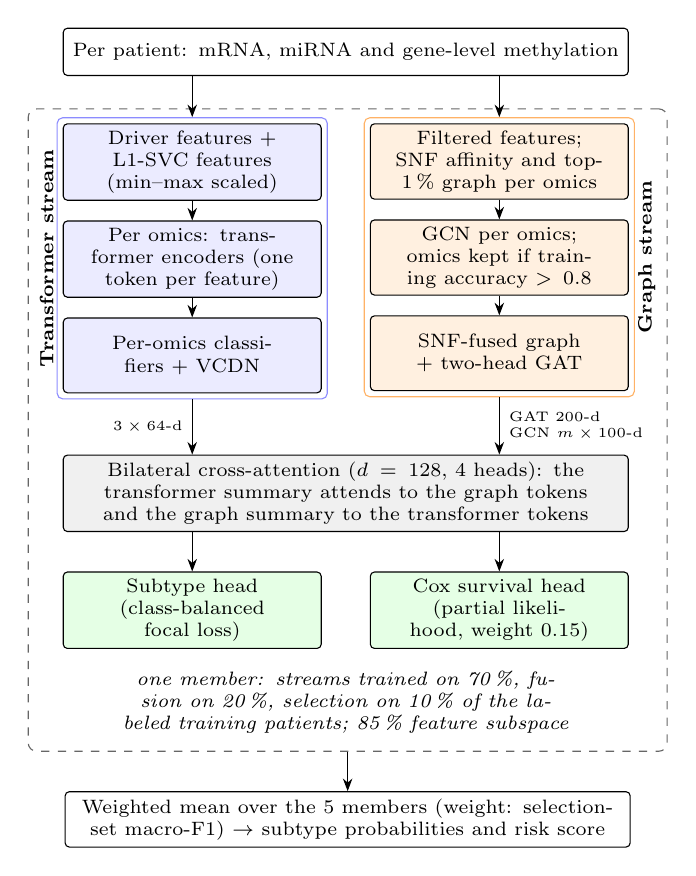
\begin{tikzpicture}[
  font=\scriptsize, >={Stealth[length=1.6mm]}, node distance=2.5mm,
  box/.style={draw, rounded corners=1.5pt, align=center, inner sep=2.5pt, minimum height=6mm},
  tbox/.style={box, fill=blue!8, text width=31mm, minimum height=9.5mm},
  gbox/.style={box, fill=orange!12, text width=31mm, minimum height=9.5mm},
  hbox/.style={box, fill=green!10, text width=31mm, minimum height=9.5mm},
  wbox/.style={box, text width=70mm},
  side/.style={font=\scriptsize\bfseries, rotate=90, inner sep=1pt}
]
\node[wbox] (in) {Per patient: mRNA, miRNA and gene-level methylation};
\node[tbox, below=6mm of in.south west, anchor=north west] (t1) {Driver features + L1-SVC features (min--max scaled)};
\node[gbox, below=6mm of in.south east, anchor=north east] (g1) {Filtered features; SNF affinity and top-1\,\% graph per omics};
\node[tbox, below=of t1] (t2) {Per omics: transformer encoders (one token per feature)};
\node[gbox, below=of g1] (g2) {GCN per omics; omics kept if training accuracy $>0.8$};
\node[tbox, below=of t2] (t3) {Per-omics classifiers + VCDN};
\node[gbox, below=of g2] (g3) {SNF-fused graph + two-head GAT};
\begin{scope}[on background layer]
  \node[fit=(t1)(t3), draw=blue!45, rounded corners=2pt, inner sep=2pt] (T) {};
  \node[fit=(g1)(g3), draw=orange!60, rounded corners=2pt, inner sep=2pt] (G) {};
\end{scope}
\node[side, anchor=south] (tl) at (T.west) {Transformer stream};
\node[side, anchor=north] (gl) at (G.east) {Graph stream};
\coordinate (fc) at (in.south |- T.south);
\node[wbox, fill=gray!12, below=7mm of fc] (f) {Bilateral cross-attention ($d=128$, 4 heads): the transformer summary
attends to the graph tokens and the graph summary to the transformer tokens};
\node[hbox, below=5mm of f.south west, anchor=north west] (h1) {Subtype head\\(class-balanced focal loss)};
\node[hbox, below=5mm of f.south east, anchor=north east] (h2) {Cox survival head\\(partial likelihood, weight 0.15)};
\coordinate (mc) at (f.south |- h1.south);
\node[below=1.5mm of mc, text width=70mm, align=center, font=\scriptsize\itshape] (ml) {one member: streams trained on
70\,\%, fusion on 20\,\%, selection on 10\,\% of the labeled training patients; 85\,\% feature subspace};
\begin{scope}[on background layer]
  \node[fit=(T)(G)(tl)(gl)(f)(h1)(h2)(ml), draw=black!60, dashed, rounded corners=3pt, inner sep=3pt] (M) {};
\end{scope}
\node[wbox, below=5mm of M] (out) {Weighted mean over the 5 members (weight: selection-set macro-F1) $\rightarrow$
subtype probabilities and risk score};
\draw[->] (in.south -| T.north) -- (T.north);
\draw[->] (in.south -| G.north) -- (G.north);
\draw[->] (t1) -- (t2);
\draw[->] (t2) -- (t3);
\draw[->] (g1) -- (g2);
\draw[->] (g2) -- (g3);
\draw[->] (T.south) -- (f.north -| T.south) node[midway, left, font=\tiny] {$3\times64$-d};
\draw[->] (G.south) -- (f.north -| G.south) node[midway, right, font=\tiny, align=left] {GAT 200-d\\GCN $m\times100$-d};
\draw[->] (f.south -| h1.north) -- (h1.north);
\draw[->] (f.south -| h2.north) -- (h2.north);
\draw[->] (M.south) -- (out.north);
\end{tikzpicture}
\caption{Ensembled Transformer-Graph Streams. One bagged member is shown (dashed box); each outer training fold trains five
members on different splits and feature subspaces, and their outputs are averaged.}
\label{fig:arch}
\end{figure}

% -------------------------------------------------------------------------------------
\section{Experimental Setup}
% sources: src/train_exact.py, external/CHANGES.md, src/report_exact.py, results/*/<cohort>_5fold_results.json
% (elapsed_minutes), .venv package versions
\emph{Protocol.} Each cohort is split by stratified 5-fold cross-validation (shuffled, seed 42) over all samples; labeled
samples are stratified by class and unlabeled samples by death event. All feature preparation (scaling, L1-SVC
selection, z-scores) is fitted on the training patients of the fold only, and every labeled sample is tested exactly
once.

\emph{Baselines.} (i) The released code of both original methods was run standalone on the same samples, folds and
per-fold features. Because both codes are purely supervised, they receive only the labeled samples. The transformer
code runs with its released defaults (Table~\ref{tab:hyper}) with one change: the epoch is chosen on a 10\,\% validation
slice of the training fold instead of on the test patients, so the code trains on 90\,\% of each training fold. The
graph code runs with its released settings on our three omics; its omics selection is applied when not all omics pass
the training-accuracy threshold (the released code tests against its four omics), and the reported model is the
selected-omics model if a selection was made and the all-omics model otherwise, as in the authors' description. Other
changes concern only file paths, the device and saving predictions. (ii) Our two streams alone, each bagged as in
Sec.~\ref{sec:bagging}.

\emph{Metrics.} Accuracy and macro-F1 are pooled over the five test folds (every labeled sample predicted once); fold
means and standard deviations are given in the text. Paired predictions are compared with the exact McNemar test
\cite{mcnemar1947}; p-values are not corrected for multiple comparisons. For survival we report Harrell's C-index
\cite{harrell1982cindex} per test fold (mean $\pm$ SD) and over the pooled out-of-fold risk scores. Patients are split
into high- and low-risk groups at the median risk of each test fold and compared with the log-rank test, a Cox hazard
ratio and the 5-year Kaplan--Meier survival, computed with lifelines \cite{davidson2019lifelines}.

\emph{Implementation.} Python 3.13, PyTorch 2.14.1 with CUDA 12.6 \cite{paszke2019pytorch}, scikit-learn 1.9.1
\cite{pedregosa2011sklearn}, snfpy 0.2.2 and lifelines 0.30.3, on one NVIDIA RTX 2000 Ada GPU (16 GB). Training the
full five-fold, five-member model took 40--109 minutes per cohort.

\begin{table}[t]
\centering
\caption{Transformer-stream settings: original paper \cite{meng2026motcs} (Sec.~4.5), released code and this work
(n.s.\ = not stated).}
\label{tab:hyper}
% sources: papers/ref_transformer_2026.pdf Sec. 4.5; external/ref_transformer_original/2.src/train_test_dg+nocdg_KIPAN.py
% (argument defaults, training loop); src/train_exact.py (our run: --trans_lr 1e-4 --trans_pretrain_epochs 50) and
% configs/cohorts.json (heads)
\footnotesize
\setlength{\tabcolsep}{4pt}
\begin{tabular}{@{}lccc@{}}
\toprule
Setting & Paper & Released code & Ours \\
\midrule
Optimiser               & Adam            & Adam          & Adam \\
Learning rate           & $10^{-5}$       & $10^{-4}$     & $10^{-4}$ \\
Batch size              & 128             & 64            & 128$^{a}$ \\
Epochs / early stop     & 100 / 50        & 50 / none     & 100 / 50 \\
Pre-training epochs     & n.s.            & 50            & 50 \\
Attention heads         & 4 (KIPAN 2)$^{b}$ & 1           & 4 (KIPAN 2)$^{b}$ \\
$d_{\mathrm{model}}$    & n.s.            & 512           & 128 \\
Feed-forward size       & n.s.            & 512           & 512 \\
Encoder layers          & n.s.            & 2             & 2 \\
Dropout                 & 0.1             & 0.1           & 0.1 \\
Epoch chosen by         & n.s.            & test accuracy & selection-set accuracy \\
\bottomrule
\multicolumn{4}{@{}p{0.97\columnwidth}@{}}{\scriptsize $^{a}$ micro-batches of 16 with summed gradients.
$^{b}$ Paper: BRCA, COAD and PRAD 4, KIPAN 2; LGG and STAD are not in the paper, and we use 4 for LGG, COADREAD and STAD.}
\end{tabular}
\end{table}

% -------------------------------------------------------------------------------------
\section{Results and Discussion}

% Sources of every number in this section (read 2026-11-08, no new files):
%   accuracy of the released codes: results/comparison_author_code/accuracy_comparison.csv
%   macro-F1 of the released codes and McNemar tests: pooled from
%     results/baselines_author_code/baseline_transformer/<cohort>/fold<k>/best_pred_total_DG.csv and
%     results/baselines_author_code/baseline_graph/<cohort>/fold<k>/test_predictions.csv (rows in the same order),
%     matched to results/final_ensembled_streams/<cohort>_predictions.csv by sample id (true labels identical)
%   our model and streams: results/final_ensembled_streams/<cohort>_5fold_results.json ("pooled_out_of_fold")
%   per-class F1: <cohort>_predictions.csv (pred_ensembled); survival: report/survival_summary.csv;
%   omics importance: report/REPORT.md ("Whole-omics importance"); enrichment: report/enrichment/enrichment_summary.csv
%   published numbers: configs/base_paper_results.json
\subsection{Comparison with the original methods}
Table~\ref{tab:main} compares the five methods on identical folds. The ensembled model has the highest pooled accuracy
on BRCA, LGG and KIPAN; on STAD it is equal to our graph stream alone (0.8542), and on COADREAD our graph stream alone
is higher (0.7609 vs.\ 0.7578, one sample). The ensembled model has the highest macro-F1 on BRCA,
LGG and COADREAD, while our graph stream alone is slightly higher on KIPAN (0.9544 vs.\ 0.9538) and STAD (0.6820 vs.\
0.6797). The fold mean $\pm$ SD of its accuracy is $0.8688\pm0.0169$ (BRCA), $0.9801\pm0.0123$ (LGG),
$0.9571\pm0.0146$ (KIPAN), $0.7577\pm0.0393$ (COADREAD) and $0.8539\pm0.0397$ (STAD) (sample SD). The released codes vary
more between folds, for example on LGG ($0.8625\pm0.1277$ for the transformer code and $0.8901\pm0.1283$ for the graph
code), mostly because of one weak fold each (accuracy 0.67 in fold~4 of the transformer code and in fold~5 of the graph
code).

The ensembled model is significantly better than the released transformer code on all five cohorts
($p\le0.037$). Against the released graph code the difference is significant on BRCA ($p=6.5\times10^{-5}$; 45 samples
correct only with our model vs.\ 14 only with the graph code), LGG ($p=5.7\times10^{-10}$; 51 vs.\ 6) and COADREAD
($p=0.040$; 53 vs.\ 33), but not on KIPAN and STAD ($p=0.11$, 0.31). Against our own graph stream alone, no difference
is significant ($p\ge0.51$): the fusion changes the accuracy by 0.0089 (BRCA), 0.0060 (LGG), 0.0020 (KIPAN), $-0.0031$
(COADREAD) and 0.0000 (STAD). Much of the advantage over the released graph code is therefore already present in the
bagged graph stream (e.g.\ 0.8599 vs.\ 0.8138 on BRCA, 0.9741 vs.\ 0.8904 on LGG and 0.7609 vs.\ 0.6957 on COADREAD),
and the contribution of the fusion itself is small.

Our transformer stream and the released transformer code both reach a low macro-F1 on BRCA (0.4469 and 0.4639),
COADREAD (0.2744 and 0.2724) and STAD (0.3125 and 0.3392), so this weakness is not caused by our implementation. A
possible reason, not tested here, is the released sample weight, which is proportional to the class share and therefore
favours large classes.

Published results were obtained with other omics, labels or a single split and are mentioned only as context. The
transformer paper reports a macro-F1 of 0.832 on BRCA \cite{meng2026motcs}, and its released code chooses the epoch on
the test patients. The graph paper reports 0.804 (BRCA), 0.992 (LGG), 0.272 (COADREAD) and 0.637 (STAD) with CNA,
methylation, mRNA and RPPA and a single 75/25 split \cite{dou2025mogcan}. Our pooled macro-F1 is higher on BRCA,
COADREAD and STAD and lower on LGG.

\begin{table*}[t]
\centering
\caption{Subtype classification on identical 5-fold splits: accuracy (Acc) and macro-F1 (mF1) pooled over the test
folds, and exact McNemar p-values of the ensembled model against each other method. Bold: best per column.}
\label{tab:main}
\footnotesize
\setlength{\tabcolsep}{4pt}
\begin{tabular}{@{}l cc cc cc cc cc@{}}
\toprule
 & \multicolumn{2}{c}{BRCA} & \multicolumn{2}{c}{LGG} & \multicolumn{2}{c}{KIPAN} & \multicolumn{2}{c}{COADREAD}
 & \multicolumn{2}{c}{STAD} \\
\cmidrule(lr){2-3}\cmidrule(lr){4-5}\cmidrule(lr){6-7}\cmidrule(lr){8-9}\cmidrule(l){10-11}
Method & Acc & mF1 & Acc & mF1 & Acc & mF1 & Acc & mF1 & Acc & mF1 \\
\midrule
Transformer method, released code \cite{meng2026motcs}
  & 0.7677 & 0.4639 & 0.8625 & 0.8552 & 0.8574 & 0.7130 & 0.6988 & 0.2724 & 0.7085 & 0.3392 \\
Graph method, released code \cite{dou2025mogcan}
  & 0.8138 & 0.7708 & 0.8904 & 0.8910 & 0.9453 & 0.9445 & 0.6957 & 0.2889 & 0.8367 & 0.6628 \\
Transformer stream alone (bagged)
  & 0.7535 & 0.4469 & 0.9024 & 0.8685 & 0.8457 & 0.7451 & 0.7019 & 0.2744 & 0.7172 & 0.3125 \\
Graph stream alone (bagged)
  & 0.8599 & 0.8191 & 0.9741 & 0.9740 & 0.9551 & \textbf{0.9544} & \textbf{0.7609} & 0.3616 & \textbf{0.8542} & \textbf{0.6820} \\
Ensembled streams (ours)
  & \textbf{0.8688} & \textbf{0.8382} & \textbf{0.9801} & \textbf{0.9815} & \textbf{0.9570} & 0.9538
  & 0.7578 & \textbf{0.3882} & \textbf{0.8542} & 0.6797 \\
\midrule
\multicolumn{11}{@{}l}{\emph{McNemar p, ours vs.:}} \\
\quad transformer code & \multicolumn{2}{c}{$2.1\times10^{-7}$} & \multicolumn{2}{c}{$1.1\times10^{-14}$}
  & \multicolumn{2}{c}{$2.2\times10^{-10}$} & \multicolumn{2}{c}{0.037} & \multicolumn{2}{c}{$7.8\times10^{-8}$} \\
\quad graph code & \multicolumn{2}{c}{$6.5\times10^{-5}$} & \multicolumn{2}{c}{$5.7\times10^{-10}$}
  & \multicolumn{2}{c}{0.11} & \multicolumn{2}{c}{0.040} & \multicolumn{2}{c}{0.31} \\
\quad transformer stream & \multicolumn{2}{c}{$1.9\times10^{-8}$} & \multicolumn{2}{c}{$2.2\times10^{-10}$}
  & \multicolumn{2}{c}{$7.7\times10^{-12}$} & \multicolumn{2}{c}{0.038} & \multicolumn{2}{c}{$3\times10^{-7}$} \\
\quad graph stream & \multicolumn{2}{c}{0.54} & \multicolumn{2}{c}{0.51} & \multicolumn{2}{c}{1.0}
  & \multicolumn{2}{c}{1.0} & \multicolumn{2}{c}{1.0} \\
\midrule
Labeled test samples & \multicolumn{2}{c}{564} & \multicolumn{2}{c}{502} & \multicolumn{2}{c}{512}
  & \multicolumn{2}{c}{322} & \multicolumn{2}{c}{343} \\
\bottomrule
\end{tabular}
\end{table*}

\subsection{Per-class behaviour}
Fig.~\ref{fig:confusion} shows the out-of-fold confusion matrices. On LGG and KIPAN every class reaches an F1 of at least
0.947. On BRCA the F1 is 0.974 for Basal, 0.900 for LumA, 0.800 for Her2, 0.769 for Normal-like and 0.748 for LumB. On
COADREAD the four larger classes reach 0.344 (COAD\_GS) to 0.871 (COAD\_MSI) and READ\_GS (6 samples) reaches 0.250 (1 of 6 correct), but
the three smallest classes (COAD\_POLE, READ\_POLE and READ\_MSI with 2 samples each) are never predicted correctly, which
limits the macro-F1 to 0.388. On STAD the POLE class (7 samples) is never predicted correctly, while the other classes
reach 0.667 (GS) to 0.967 (EBV). These classes have only 1--6 training samples per fold, of which each member's streams
see about 70\,\%.

\begin{figure*}[t]
\centering
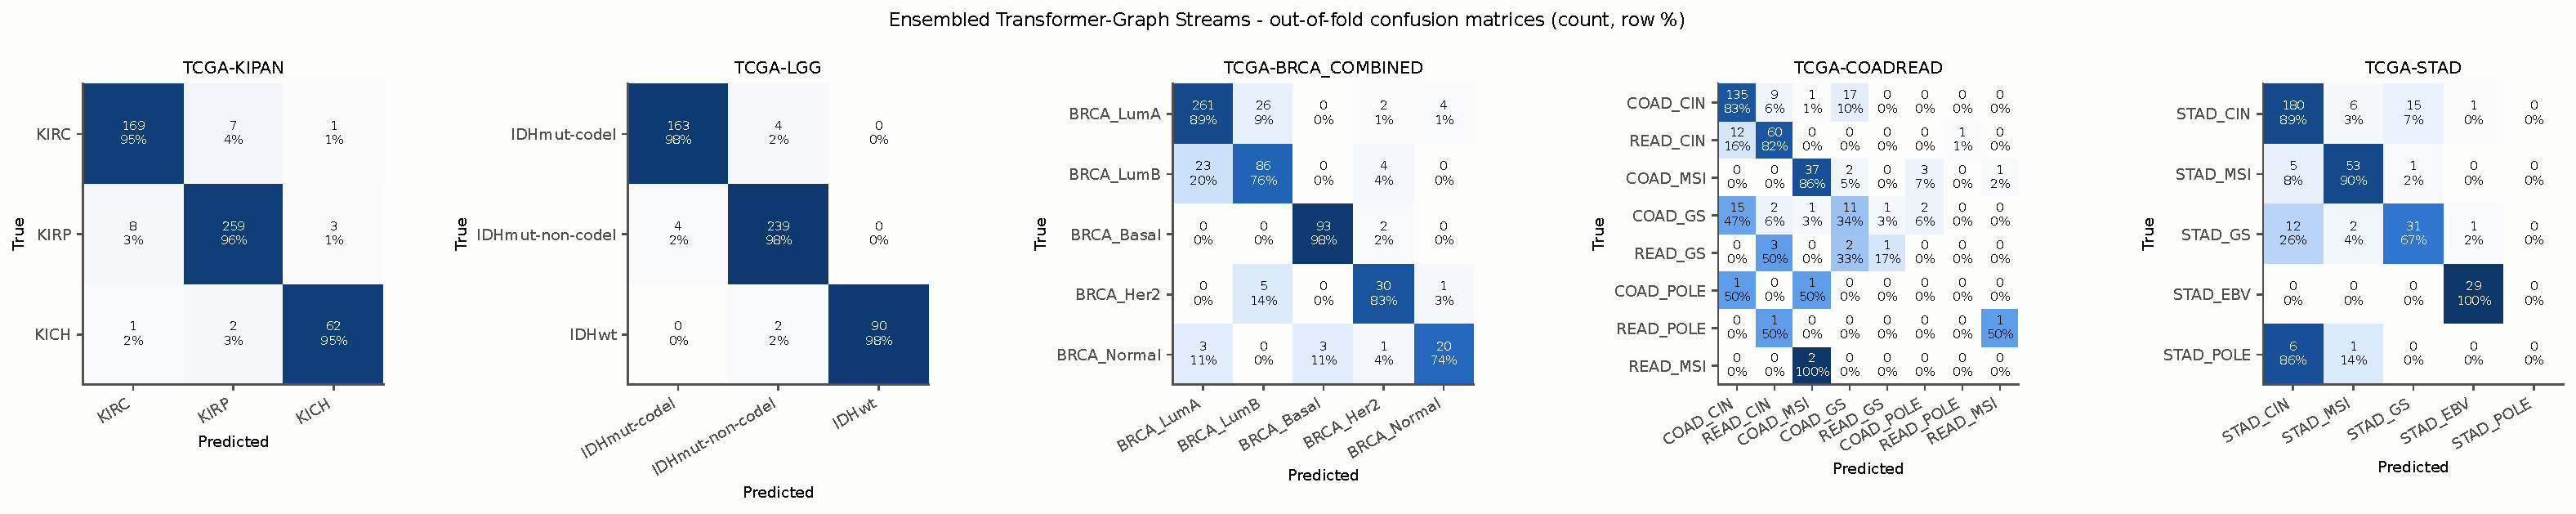
\includegraphics[width=\textwidth]{figures/fig2_confusion_ensembled.pdf}
\caption{Out-of-fold confusion matrices of the ensembled model.}
\label{fig:confusion}
\end{figure*}

\subsection{Survival prediction}
\label{sec:surv}
Table~\ref{tab:surv} and Fig.~\ref{fig:km} summarise the Cox head. The fold-mean C-index ranges from 0.765 (LGG) to
0.532 (STAD). The median-risk split separates survival significantly on KIPAN (hazard ratio 2.77,
$p=3.3\times10^{-6}$), LGG (2.75, $p=3.7\times10^{-8}$) and BRCA (1.66, $p=0.025$), but not on COADREAD
($p=0.13$) or STAD ($p=0.24$), where the confidence intervals of the hazard ratio include 1. The C-index over the pooled
out-of-fold risk scores is lower than the fold mean on every cohort (KIPAN 0.640, LGG 0.749, BRCA 0.649, COADREAD 0.561,
STAD 0.523), because the risk scores of different folds are not calibrated to a common scale. The STAD C-index includes
the three deaths without a survival time (Sec.~\ref{sec:data}); without them, computed from the same risk scores, it is
$0.544\pm0.039$ over the folds and 0.537 pooled, so the conclusion that survival prediction is weak on STAD does not
change. The model itself was trained with these three samples.
% source: inline recomputation 2026-11-09 (owner yes, no files): folds rebuilt with StratifiedKFold(5, shuffle, seed 42)
% as in src/train_exact.py, reproducing all five stored fold C-indices; C-index as compute_c_index in
% src/models/ensembled_streams.py on stad_predictions.csv without TCGA-3M-AB47, TCGA-BR-7851, TCGA-IN-A6RO
% (fold values 0.5486, 0.5261, 0.5194, 0.5086, 0.6169; SD with denominator 5).

\begin{table}[t]
\centering
\caption{Survival prediction of the ensembled model. C-index: mean $\pm$ SD over the five test folds (SD with
denominator 5). High vs.\ low risk: median split of the predicted risk in each test fold; samples with OS time $\le0$
excluded.}
\label{tab:surv}
\resizebox{\columnwidth}{!}{%
\begin{tabular}{@{}l c c c c c@{}}
\toprule
Cohort & Samples / deaths & C-index & Log-rank $p$ & HR (95\,\% CI) & 5-yr OS high / low \\
\midrule
BRCA     & 616 / 80  & $0.662\pm0.033$ & 0.025              & 1.66 (1.06--2.61) & 72.9 / 85.6\,\% \\
LGG      & 505 / 124 & $0.765\pm0.094$ & $3.7\times10^{-8}$ & 2.75 (1.89--4.00) & 45.0 / 78.4\,\% \\
KIPAN    & 507 / 94  & $0.659\pm0.070$ & $3.3\times10^{-6}$ & 2.77 (1.77--4.33) & 68.3 / 84.4\,\% \\
COADREAD & 332 / 72  & $0.564\pm0.046$ & 0.13               & 1.43 (0.89--2.28) & 55.9 / 68.1\,\% \\
STAD     & 360 / 140 & $0.532\pm0.044$ & 0.24               & 1.22 (0.88--1.70) & 32.0 / 42.9\,\% \\
\bottomrule
\end{tabular}}
\end{table}

\begin{figure*}[t]
\centering
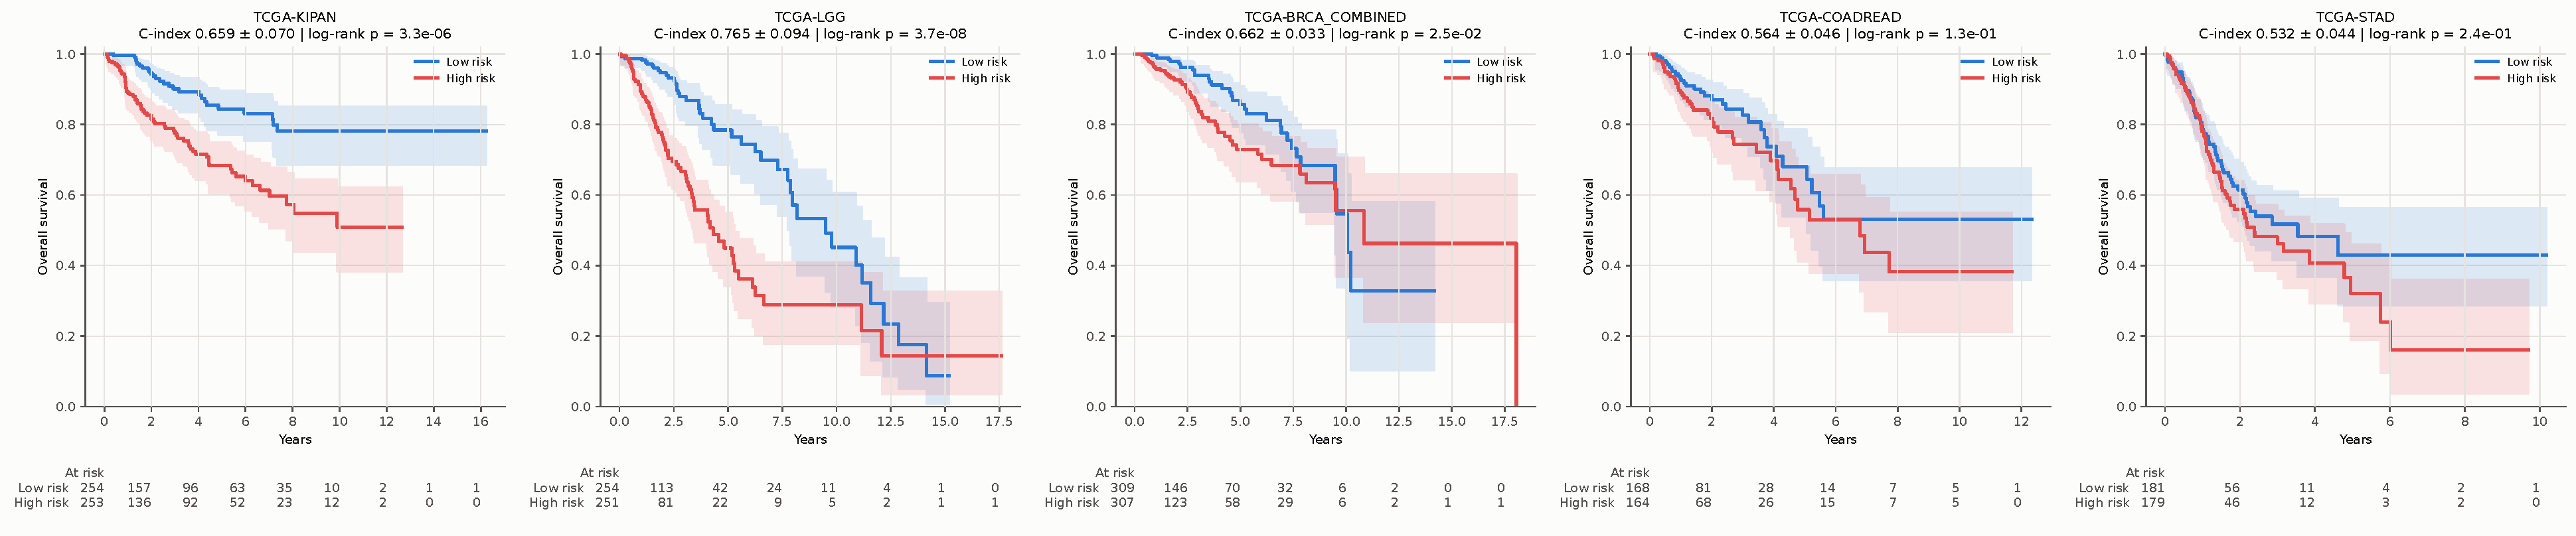
\includegraphics[width=\textwidth]{figures/fig3a_kaplan_meier.pdf}
\caption{Kaplan--Meier curves of the high- and low-risk groups (median split of the predicted risk in each test fold).}
\label{fig:km}
\end{figure*}

% Sources (read 2026-11-09, no new files): report/REPORT.md (whole-omics table);
%   report/<cohort>_top30_{subtype,survival}_ensembled_{mrna,mirna,meth}.csv (rank, kind = driver / l1svc, mean drop over
%   all 25 members with 0 for members without the feature, used_by_members); driver share of the inputs = drivers /
%   (drivers + 0.85 x mean L1-SVC count over the folds, train_<cohort>.log); report/enrichment/enrichment_summary.csv
%   and enrichment_info.json (20 gene lists = mRNA and methylation x 2 tasks x 5 cohorts; 14 with a term at FDR < 0.05).
\subsection{Omics importance and biological interpretation}
After training, we set all transformer-stream inputs of one omics to zero in the test fold, leaving the graph stream's
inputs unchanged, and measured the drop in performance (Fig.~\ref{fig:omics}). The largest macro-F1 drops of the
ensembled model come from mRNA on BRCA (0.229) and COADREAD (0.105), from methylation on STAD (0.193) and LGG (0.100),
and from miRNA on KIPAN (0.044). The standard deviations over the 25 members are large (0.5 to 2.5 times these means), and the
C-index drops are at most 0.043.

\emph{Single features.} Following the transformer method \cite{meng2026motcs}, each transformer-stream input was set to
zero in the test fold, one at a time, and the features of each omics were ranked by the mean drop in the ensembled
macro-F1 (subtype) or C-index (survival) over the 25 members, counting 0 for members whose feature subspace did not
contain the feature. Single features change these metrics by at most 0.007, so the rankings describe small effects.
Driver features are not over-represented at the top: they make up 3--30\,\% of the top-30 mRNA and methylation subtype
lists, and in every cohort this is less than their share of the inputs a member receives (23--47\,\%). The top miRNAs
are mostly driver miRNAs (70--100\,\%), in line with their 86--93\,\% share of the miRNA inputs.

Several top-ranked features are known markers of the classes they separate (Table~\ref{tab:bio}). In LGG, the subtype
lists contain IDH1 and ATRX expression and IDH2 methylation; IDH mutation and 1p/19q co-deletion define the three LGG
classes, and ATRX loss is typical of the IDH-mutant non-codeleted class \cite{tcga2015lgg}. In BRCA, FOXC1 and ESR1, two of the PAM50 genes \cite{parker2009pam50}, are among
the top subtype mRNA features (ranks 8 and 13), and FOXC1 is also the 7th survival mRNA feature. In KIPAN, the lists contain VHL
expression and SETD2 methylation, two genes frequently inactivated in clear-cell renal carcinoma (KIRC)
\cite{tcga2013kirc}. In STAD the top subtype methylation feature is EPM2AIP1, which shares a promoter CpG island with
MLH1 \cite{damaso2018mlh1}; MLH1 promoter hypermethylation underlies most sporadic MSI tumours in gastric and colorectal
cancer \cite{tcga2012crc,tcga2014stad}. In COADREAD, in contrast, MLH1 expression ranks only 44th for the subtype and
16th for survival. EPM2AIP1 and MLH1 were selected by the L1-SVC, not taken from the driver lists. In STAD, the subtype lists also contain RHOA expression and
CDH1 methylation, two genes whose mutations are enriched in the genomically stable (GS) class \cite{tcga2014stad}. These are
associations only: the features are expression or methylation values, not the mutations that define the classes, and a
high rank does not show how the model uses a feature.

\emph{Pathway enrichment.} The top-30 mRNA and methylation genes of each cohort and task were tested for GO Biological
Process 2025 and KEGG 2021 enrichment with Enrichr through GSEApy 1.3.2 \cite{kuleshov2016enrichr,fang2023gseapy}
(FDR $<0.05$, Enrichr default background); 13 of the 20 lists have at least one significant term. Examples are the KEGG
glioma pathway for the LGG subtype methylation genes (PTEN, BRAF, PIK3R1, PLCG1; adjusted $p=1.8\times10^{-4}$), the
KEGG gastric cancer pathway for the STAD subtype methylation genes (SMAD2, APC, CDH1, AXIN2; $p=0.0020$), the KEGG
pathways in cancer for the BRCA survival methylation genes (CCND1, ERBB2, GNAS, KLK3, KRAS, RUNX1; $p=0.0036$) and
the regulation of double-strand break repair by homologous recombination for the KIPAN subtype methylation genes
(MBTD1, SETD2, TRRAP, ARID2; $p=0.0019$). The COADREAD lists give only three significant terms, none of them a cancer
pathway. About three quarters of the gene hits behind the significant terms (766 of 986)
are driver genes, which are cancer genes by construction, so enrichment of cancer pathways is partly expected. With lists of at most 30 genes and the default
background, this analysis is exploratory.

\begin{table}[t]
\centering
\caption{Known class markers among the top-30 features of the ensembled model (rank in the subtype list unless stated;
D = driver feature, S = selected by L1-SVC).}
\label{tab:bio}
\footnotesize
\setlength{\tabcolsep}{3pt}
\begin{tabular}{@{}l l c p{3.6cm}@{}}
\toprule
Cohort & Feature (omics, rank) & Src & Known role \\
\midrule
LGG      & IDH1 (mRNA, 4)                    & D & IDH status defines the classes \cite{tcga2015lgg} \\
         & IDH2 (meth., 14)                  & D & IDH status \cite{tcga2015lgg} \\
         & ATRX (mRNA, 27)                   & D & loss typical of IDHmut-non-codel \cite{tcga2015lgg} \\
BRCA     & FOXC1 (mRNA, 8; survival 7)       & S & PAM50 gene \cite{parker2009pam50} \\
         & ESR1 (mRNA, 13)                   & D & PAM50 gene \cite{parker2009pam50} \\
KIPAN    & VHL (mRNA, 30)                    & D & inactivated in KIRC \cite{tcga2013kirc} \\
         & SETD2 (meth., 10)                 & D & mutated in KIRC \cite{tcga2013kirc} \\
STAD     & EPM2AIP1 (meth., 1)             & S & shares the MLH1 CpG island \cite{damaso2018mlh1} \\
         & RHOA (mRNA, 17)                   & D & mutations enriched in GS \cite{tcga2014stad} \\
         & CDH1 (meth., 28)                  & D & mutations enriched in GS \cite{tcga2014stad} \\
\bottomrule
\end{tabular}
\end{table}

\begin{figure}[t]
\centering
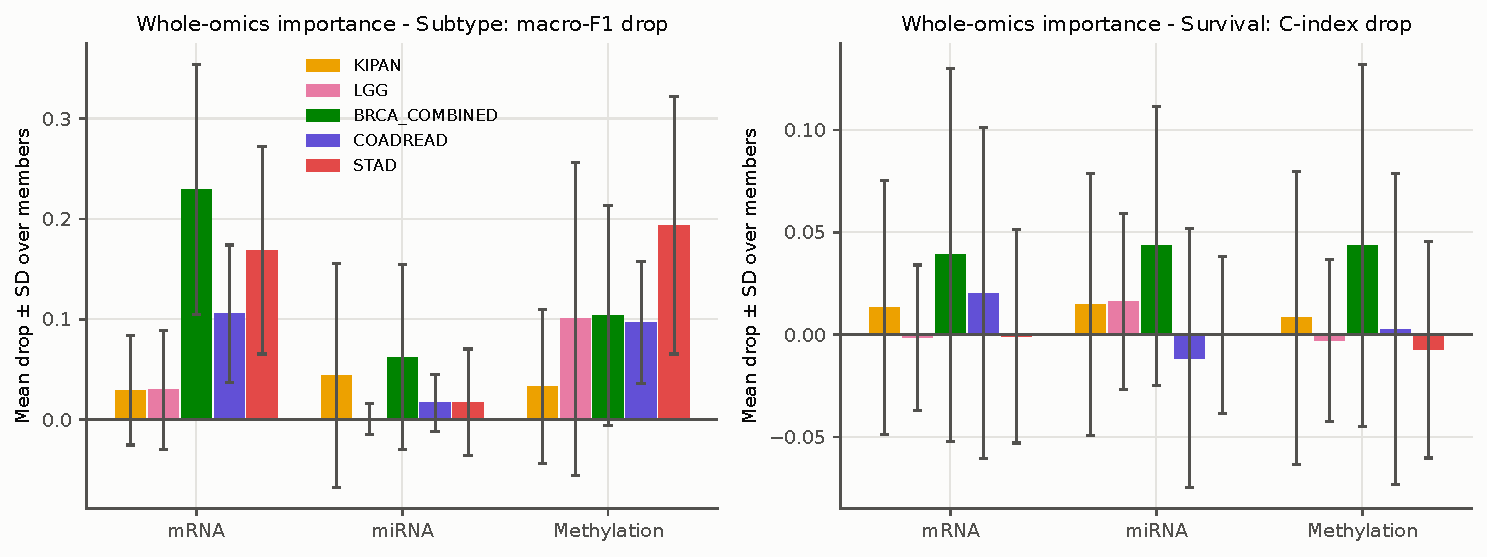
\includegraphics[width=\columnwidth]{figures/fig4_whole_omics_importance.pdf}
\caption{Whole-omics importance: drop in performance when all transformer-stream inputs of one omics are set to zero in
the test fold (mean $\pm$ SD over the 25 ensemble members).}
\label{fig:omics}
\end{figure}

\subsection{Discussion}
The two streams are not equally strong. The graph stream alone is already close to the ensembled model on every cohort,
while the transformer stream is weaker, especially in macro-F1 on the imbalanced cohorts (BRCA, COADREAD, STAD). The
fusion therefore mostly refines the graph stream: it adds 0.0089 accuracy on BRCA, little on LGG and KIPAN, nothing on
STAD and loses one sample on COADREAD, and none of these differences is significant. On COADREAD it raises the
macro-F1 from 0.3616 to 0.3882: the F1 of READ\_GS (one sample now correct) rises from 0 to 0.250 and that of READ\_CIN
from 0.712 to 0.811, while that of COAD\_GS falls from 0.484 to 0.344. The clear and significant
improvements over the released graph code on BRCA, LGG and COADREAD come largely from training the graph method as a
bagged stream, not from the fusion. We see two benefits of the fused model beyond accuracy: its accuracy is at most one
sample below the better stream on every cohort, and it gives one model for both subtype and survival, with a
significant median-risk separation on three cohorts. Its survival performance is weak on COADREAD and STAD, the two cohorts with the smallest sample sizes and,
for COADREAD, eight partly tiny classes. A stronger transformer stream, for example with a class-balanced sample weight,
may increase the value of the fusion, but this would change the published method and is left to an ablation study.

\subsection{Limitations}
(i) All results come from internal 5-fold cross-validation with one random split seed; no external cohort was used, and
cross-validation was not repeated with other seeds.
(ii) The three COADREAD classes with 2 samples and the STAD POLE class (7 samples) were never predicted correctly, and
READ\_GS (6 samples) only once; macro-F1 on these cohorts mainly reflects this.
(iii) Survival prediction is weak on COADREAD and STAD; three STAD deaths without a recorded survival time were assigned
time 0 and used in training (Sec.~\ref{sec:data}); without them the STAD C-index is 0.544 instead of 0.532.
(iv) The metastatic samples of five patients with a primary sample were removed (Sec.~\ref{sec:data}); the remaining
samples are from different patients.
(v) Methylation gene values were imputed once before the cross-validation split. The step uses no labels, and it affects
0.015--0.042\,\% of the methylation values.
(vi) The transformer stream uses $d_{\mathrm{model}}=128$ instead of the released 512, and the cancer-specific driver lists
were rebuilt by us because the original rule is not published.
(vii) The graph method was published with CNA, methylation, mRNA and RPPA; here it uses mRNA, miRNA and methylation.
(viii) Omics importance masks only the transformer-stream inputs, enrichment uses the Enrichr default background, and
p-values are not corrected for multiple comparisons.
(ix) Five members per fold make training slower than a single model (40--109 minutes per cohort on one GPU).

% -------------------------------------------------------------------------------------
\section{Conclusion}
We combined two published multi-omics subtype classifiers, a driver-aware transformer and a patient-graph network, as
unchanged streams of one model with bilateral cross-attention fusion, joint subtype and Cox survival heads and bagging
over disjoint stream, fusion and selection sets. On five TCGA cohorts, with both original codes re-run on identical
folds, the ensembled model reached the highest pooled accuracy on BRCA, LGG and KIPAN, tied with its own graph stream
on STAD and was one sample behind it on COADREAD. It was significantly better than
the released transformer code on all cohorts and than the released graph code on BRCA, LGG and COADREAD. Its
difference from its own bagged graph stream was small and not significant. Its risk score separated survival significantly on KIPAN, LGG and
BRCA but not on COADREAD and STAD. Its top-ranked features include known class markers such as IDH1 and ATRX in LGG,
VHL and SETD2 in KIPAN, FOXC1 and ESR1 in BRCA and EPM2AIP1 in STAD, although single features have small effects.
Future work should test the model on external cohorts, repeat the cross-validation with several seeds, and quantify the
contribution of each component in ablation studies.

\section*{Data and Code Availability}
All data are public: TCGA omics and survival from the UCSC Xena TCGA hub \cite{goldman2020xena} and subtype labels from
cBioPortal \cite{cerami2012cbioportal,gao2013cbioportal}; the checksums of the downloaded files are recorded in our code
repository. Our code for preprocessing, training, evaluation and the baseline runs, including a list of every change made
to the original codes, will be made available \tocheck{add repository URL}. The graph method's code is released under
the MIT licence. The transformer method's repository has no licence file, so we do not redistribute it and refer to the
authors' repository instead.

\bibliographystyle{IEEEtran}
\bibliography{refs}

\end{document}
